% for landscape posters, use "a4paper, landscape"
\documentclass[a4paper]{article}
\usepackage{better_poster}


% ---- fill in from here
% poster size - this will scale the poster to the given size.
% for landscape posters add ", landscape" to the postersize command.
\postersize{a0paper}

% authors
\title{Is the Linear Correlation Between Classification and Rotation/Jigsaw Prediction Model-Invariant?}
\author{Callum Koh}

% type of poster: [exp]erimental results, [methods], [theory]
% Disclaimer: the original classification had "study" and "intervention" as separate categories. I group them under experimental results.
\newcommand\postertype{imperialblue} % [exp],[methods],[theory]

\begin{document}

% main point of your study
\makefinding{
There is a \textbf{Strong Linear Correlation}
\\between \textbf{Image Classification} Accuracy
\\and \textbf{Jigsaw Solving/Rotation Prediction} Accuracy,
\\for \textbf{Almost All} Classification Models
}



% the main text of your poster goes here
\makemain{
    % you can have 1 or 2 columns
    \raggedcolumns
    \begin{multicols}{2}
        \section{Intro}
        \vspace{-0.3cm}
        \begin{compactitem}
            \item In real world, classifier will encounter data different from training.
            \item Will likely perform poorly.
            \item Need samples of this data with labels for improvement.
            \item Adding labels to images is laborious.
            \item \textbf{Can gauge classification accuracy from rotation or jigsaw prediction.}
        \end{compactitem}
        \begin{compactitem}
            \item \textbf{Linear relationship only shown using one model for one dataset.}
            \item \textbf{Must be tested with one dataset and many models.}
        \end{compactitem}
        \vspace{0.34cm}
        \begin{compactitem}
            \item CIFAR-10 dataset has 60,000 images, 1 of 10 unique objects in each.
            \item Includes planes, frogs, boats, etc.
        \end{compactitem}
        \vspace{-0.4cm}
        \section{Method}
        \vspace{-0.3cm}
        \begin{compactitem}
            \item[1.] Use CIFAR-10 dataset,
            \item[2.] Take pretrained image classifier,
            \item[3.] Fix weights of all layers,
            \item[4.] Train new fully-connected layer for rotation/jigsaw prediction,
            \item[5.] Test classification and rotation/jigsaw on corrupted CIFAR-10 datasets,
            \item[6.] Repeat for 16 other models.
        \end{compactitem}
        \vspace{0.3cm}
        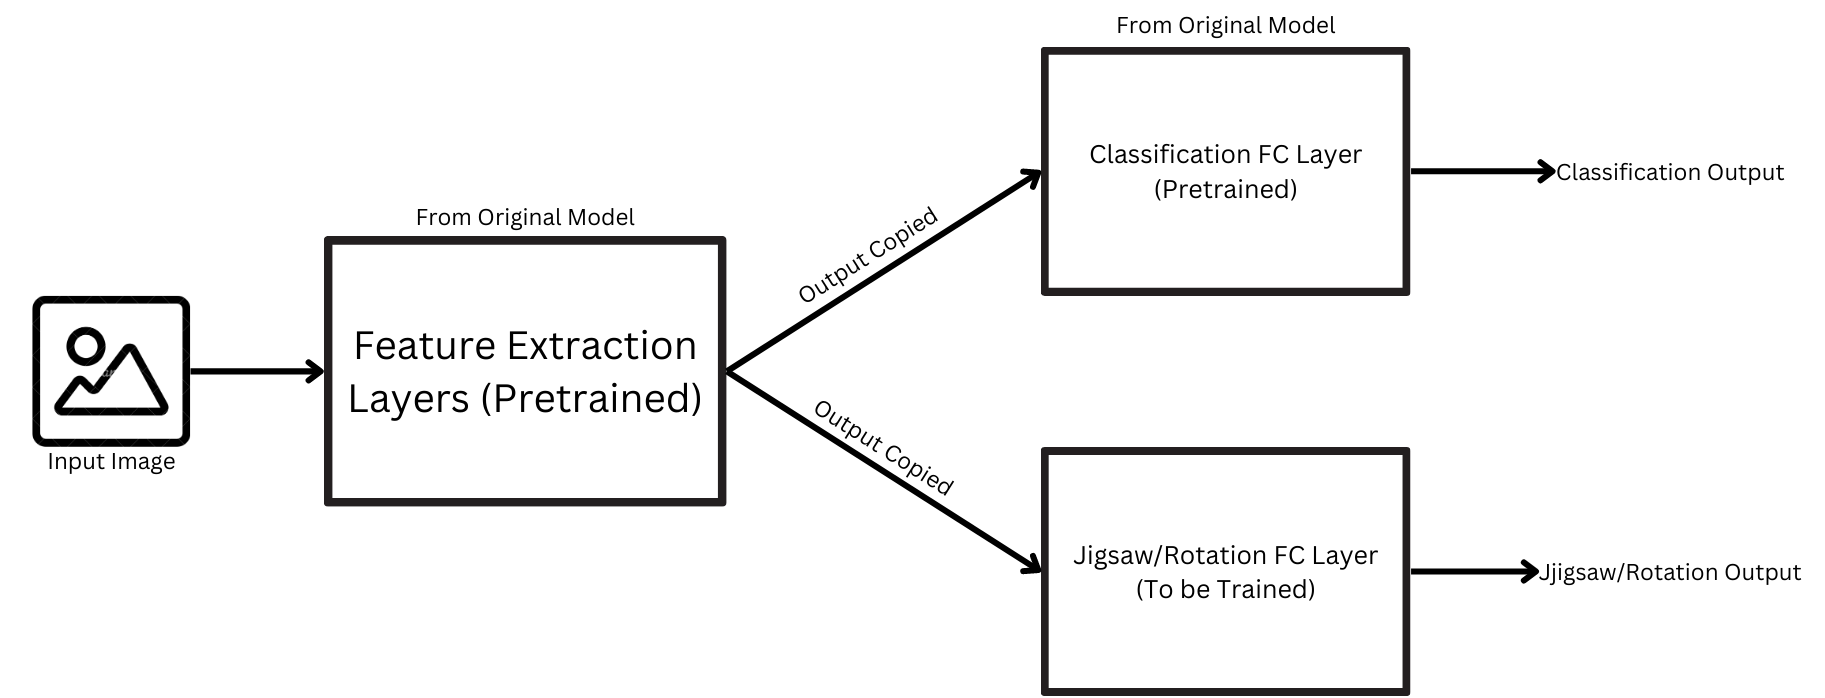
\includegraphics[scale=0.145]{images/diagram.png}
        
    % this determines where your columns will be separated
    \columnbreak

        \section{Results}
        \vspace{-0.3cm}
        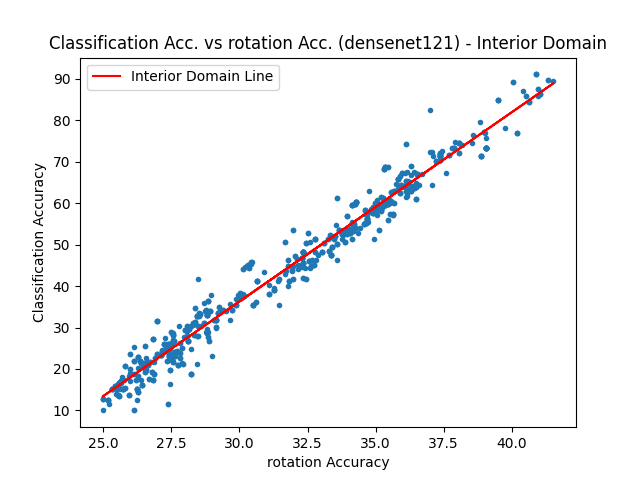
\includegraphics[scale=0.44]{images/sample1.png}
        \begin{compactitem}
            \item \textbf{Linear correlation on both tasks and both domains}, \textit{for all but one model.}
            \item Even simplest models showed medium to strong fit.
            \item Linear Fit in Interior Domain doesn't always hold in Exterior Domain.
        \end{compactitem}
        \vspace{-0.4cm}
        \section{Future Work}
        \vspace{-0.3cm}
        \begin{compactitem}
            \item Test more classifiers.
            \item Apply method to other datasets e.g: ImageNet, COCO, MNIST, etc.
            \item Test other self-supervised methods eg: image colourisation.
        \end{compactitem}
        \vspace{0.3cm}
        \includegraphics[scale=0.145]{images/diagram1.png}
    
    \end{multicols}
}
% If you have extra figures or data to show
\makeextracolumn{
    \begin{flushleft}
    Linear Classifier - Jigsaw (Simplest)
    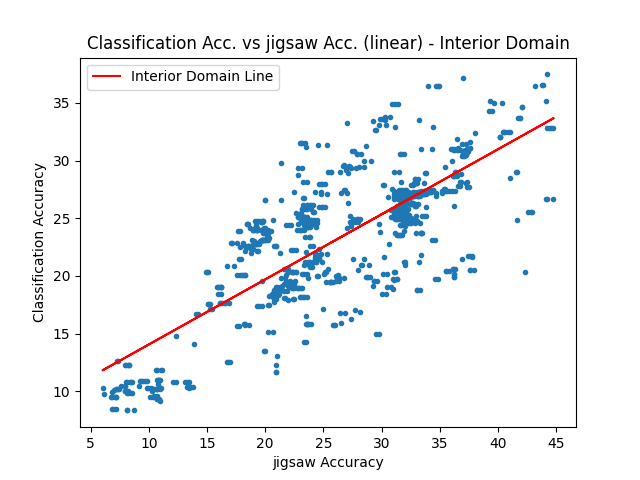
\includegraphics[scale=0.16]{images/sample3.png}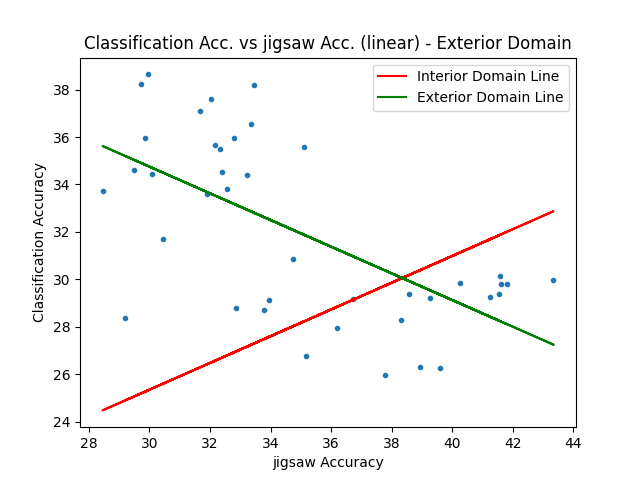
\includegraphics[scale=0.16]{images/sample2.png}
    LeNet5 - Jigsaw
    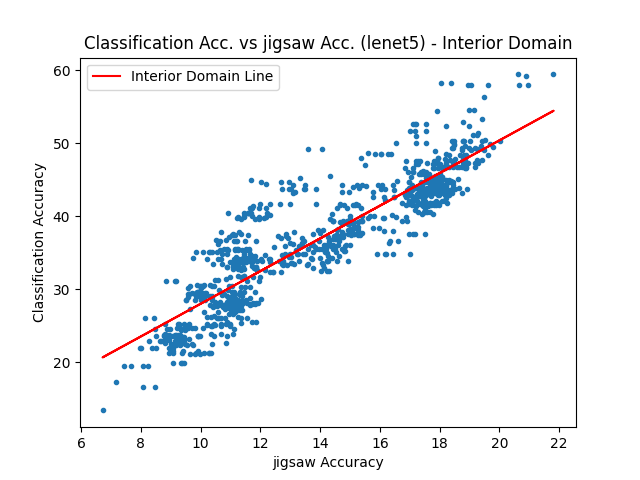
\includegraphics[scale=0.16]{images/sample8.png}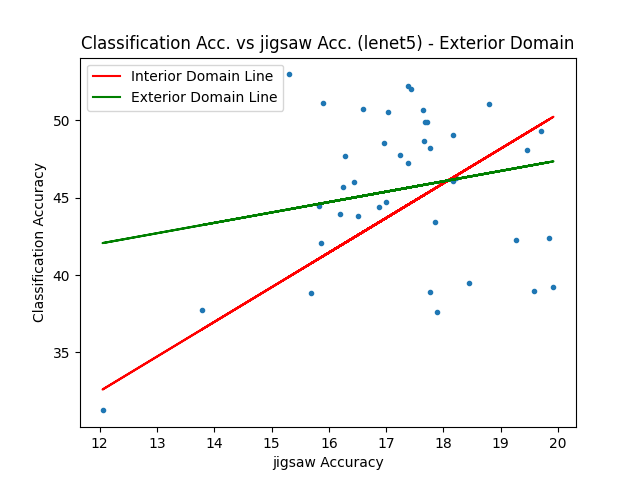
\includegraphics[scale=0.16]{images/sample9.png}
    ShuffleNet - Rotation
    \includegraphics[scale=0.16]{images/sample10.png}\includegraphics[scale=0.16]{images/sample11.png}
    Inception\_v3 - Rotation
    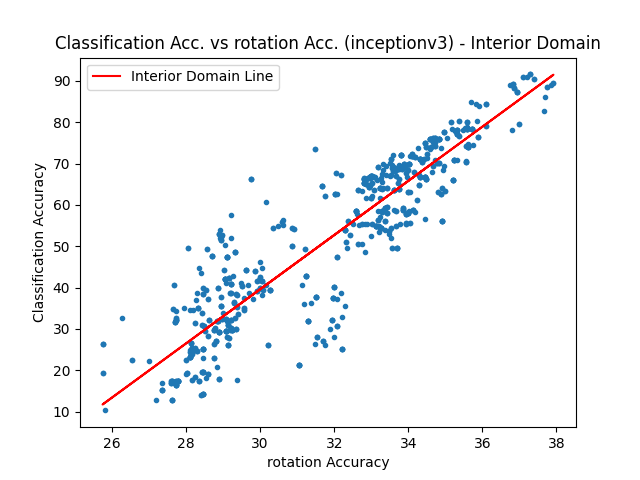
\includegraphics[scale=0.16]{images/sample4.png}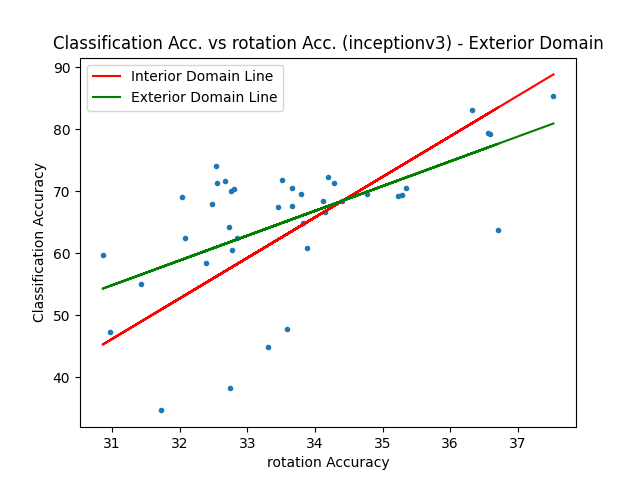
\includegraphics[scale=0.16]{images/sample5.png}
    DenseNet169 - Jigsaw
    \includegraphics[scale=0.16]{images/sample12.png}\includegraphics[scale=0.16]{images/sample13.png}
    ResNet1202 - Jigsaw (Most Complex)
    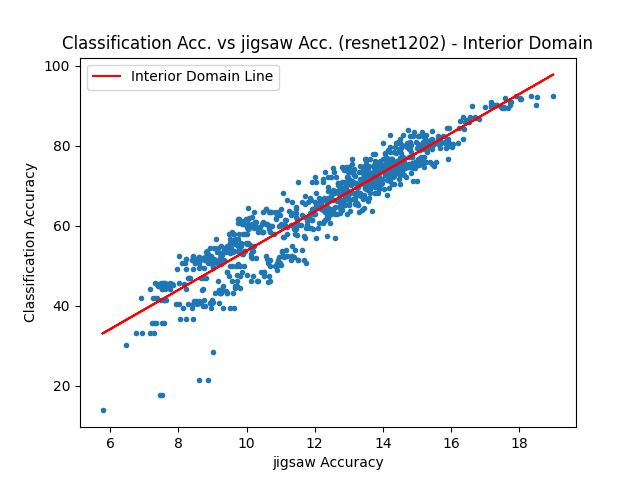
\includegraphics[scale=0.16]{images/sample6.png}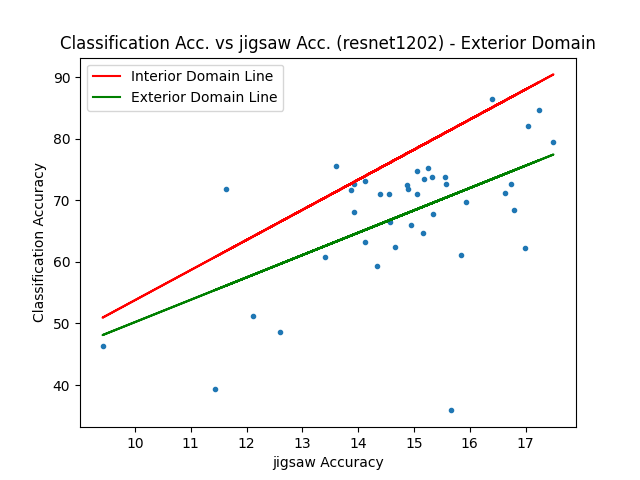
\includegraphics[scale=0.16]{images/sample7.png}

    \vspace{0.3cm}
    Interior Domain = Modified versions of original dataset for model training. Also includes original dataset.
    
    Exterior Domain = Variants of original dataset eg: CIFAR-10.1.

    \end{flushleft}
}

% footer
% generate qr code from https://www.qr-code-generator.com/ and replace qr_code.png
% default: barcode on the left
\makefooter{images/uni_logo1.png}{images/paperqr.png}
\end{document}